\chapter{Automating the Deployment of Virtual Networks} \label{chap:4}
    \epigraph{One of my most productive days was throwing away 1,000 lines of code.}{\textit{Ken Thompson}}

    \section{High Level Overview}
        As seen in chapter \ref{chap:3}, bringing a virtual network up entails an organizational overhead that is not easily handled. That is why we have developed a complete software system capable of handling these intricacies in an automatic fashion. Then, a user need only provide a \textit{graph} describing the desired topology and our project will be able to read, interpret and instantiate said network.\\

        Due to its simple yet rich syntax, we have decided to leverage the \textit{Python} \cite{bib:python} programming language to develop the entire system. We will be using version \textit{3.x} given \textit{python's} \textit{2.7} release has been deprecated as of \textit{January 2021}. One of the external dependencies we will make use of is the \textit{NetworkX} \cite{bib:networkx} network analysis module. This software bundle was recommended by the research group we have collaborated with and it is distributed as a \textit{python package}. Thus, we felt even more inclined towards \textit{python}. Given we will interact with the \textit{docker engine} through its \textit{CLI API}, its use will not impose any restrictions on our choice either. This implies that we have nothing more than reasons supporting the use of \textit{python} for our development.\\

        \subsection{External Dependencies}
            One of the main objectives pursued throughout the development was reducing the number of external dependencies to the maximum extent. We did manage to only require the presence of \textit{docker}, \textit{iproute2} and \textit{python3} for an initial and fully functional version. Not leveraging \textit{NetworkX} implied we had to manually route all the nodes within the network, which amounted to be a rather complex task. Due to the research group's suggestions we settled on taking advantage of \textit{NetworkX} for both modeling the different topologies and routing them. Then, we have designed two independent solutions that accomplish the same task. One of them \textbf{does not} require \textit{NetworkX} whist the other one \textbf{does}. The reasoning behind including a dependency that is not strictly needed is that it greatly simplifies our code and it will surely avoid some of the most common pitfalls our own solution can incur into under complex circumstances.\\

            The following enumeration briefly explains the use of each of the required dependencies. Please bear in mind that the installation instructions for each of them are detailed in the document's appendix.\\

            \begin{enumerate}
                \item \textbf{\textit{Python3}:} With \textit{python3} being an interpreted language, we need to make use of the interpreter that is going to execute our code.
                \item \textbf{\textit{Docker}:} The different nodes in our network are modeled as \textit{docker containers}, which implies we indeed depend on \textit{docker} for making our system work.
                \item \textbf{\textit{iproute2}:} We need the \textit{iproute2} suite of tools to manage the virtual networking infrastructure ``gluing'' all our nodes together.
                \item \textbf{\textit{NetworkX}:} As explained above, we \textit{are not forced} to use \textit{NetworkX} and we have developed a version that does not depend on it at all. Nonetheless, it does simplify big portions of code and so we decided to include it in our final, sharper version.
                \item \textbf{\textit{Matplotlib}:} \textit{NetworkX} is capable of graphically representing our topologies through \textit{graphs}. In order to ``draw them'', \textit{NetworkX} depends on the \textit{matplotlib} module we have also installed as a dependency. This module is however \textbf{not mandatory}: they rest of the program will work as intended, it will just be unable to graphically represent the topology. In a later chapter we will devote our time to looking into a \textit{proof of concept} we have developed. Said experiment generates a series of time-tagged events that our program is capable of representing as a regular graph. The lack of the \textit{matplotlib} module implies this graph will not be available either. All in all, it is up to the user to decide whether they want this functionality or not: the program itself will carry out is primary task either way.
                \item \textbf{\textit{Docker Python SDK}:} We \textbf{have not} used the \textit{docker python SDK} (Software Development Kit) in our project. We have decide to leverage \textit{docker's} \textit{CLI} interface from our code through calls to \texttt{os.system()}. However, someone deciding to use our project as a basis for something else might feel more comfortable interacting with \textit{docker} through a pure-\textit{python} \textit{API} (Application Programming Interface). Changing our code to work in said fashion is a rather simple task should it have to be done.
            \end{enumerate}

        \subsection{User Manual} \label{sec:user-manual}
            Throughout the development of our tool we have tried to simplify the use of the project as much as possible. The end result is a user-side workflow that only requires them to import a single project module to which they \textbf{must} provide a \textit{NetworkX graph}. After doing so, they will be presented with a simple \textit{CLI} letting them modify the currently live virtual network.\\

            \paragraph{User Permissions}
                Given the project will make use of \textit{iproute2} the program needs to be run with administrative privileges (i.e. prepended by \texttt{sudo}). Even though this is the easiest approach and everything will ``just work'' it does have some security implications (mainly command injection) we will showcase in the appendix. Instead of choosing to run the entire blob of code as \textit{root} we can also grant certain capabilities to the user who is to run the code, namely the \textit{NET\_ADMIN} capability (the same we need to grant containers). We should also mention that the user running the program must be able to interact with the \textit{docker engine}. This can be ensured by adding said user to the \textit{docker group} within the system, even though \textit{root} will also be able to interact with and manage containers. This paragraph is intended as a warning, please refer to the appendix for a deeper discussion.\\

            Depending on how the users decide to provide the required \textit{graph} they might need to import additional modules. If they have stored a live graph (i.e. an instance of a graph) as a \textit{pickle} \cite{bib:python-pickle} they will then need to import the \textit{pickle} module to \textit{un-pickle} the graph, for instance. In our examples we will define the graphs ``on-the-fly'', which requires us to import \textit{networkx} itself. Listing \ref{lst:sample-topology-graph} shows how one would define the topology found on figure \ref{fig:sample-topology} as a \textit{networkx} graph.\\

            \begin{lstlisting}[language = python, caption = Defining the Sample Topology as a \textit{networkx} Graph., label = lst:sample-topology-graph]
                # Import the networkx module so that we can define a graph.
                import networkx

                # Instantiate the netowrkx.Graph class.
                sample_net = networkx.Graph(net = 'Sample Topology')

                # Add host H-A-1 and the bridge for subnet A.
                sample_net.add_node('h-a-1', type = 'node')
                sample_net.add_node('subnet-a-brd', type = 'bridge', subnet = '10.0.0.0/24')

                # Add host H-B-1 and the bridge for subnet B.
                sample_net.add_node('h-b-1', type = 'node')
                sample_net.add_node('subnet-b-brd', type = 'bridge', subnet = '10.0.1.0/24')

                # Add the R-A-B router with NO firewall rules.
                sample_net.add_node('r-a-b', type = 'router', fw_rules = {})

                # Connect H-A-1 to the bridge for subnet A.
                sample_net.add_edge('h-a-1', 'subnet-a-brd')

                # Connect H-B-1 to the bridge for subnet B.
                sample_net.add_edge('h-b-1', 'subnet-b-brd')

                # Connect router R-A-B to both bridges.
                sample_net.add_edge('subnet-a-brd', 'r-a-b')
                sample_net.add_edge('subnet-b-brd', 'r-a-b')
            \end{lstlisting}

            \subsubsection{Creating Well-formed Graphs} \label{sec:good-graphs}
                Our tool expects the nodes on a \textit{networkx} graph to adhere to certain constraints so that it can assemble the requested topology. Given the bi-directional nature of network links (data is sent in both directions), we have decided to model our networks as \textbf{undirected graphs}. Then, these will always be composed by a set of \textit{nodes} interconnected by a set of \textit{edges}. The types of nodes one can use are listed on table \ref{tab:node-types}.\\

                \begin{table}
                    \centering
                    \begin{tabular}{|c|c|}
                        \hline
                        \textbf{Node Type} & \textbf{Description}\\
                        \hline
                        \textit{node} & A regular host.\\
                        \hline
                        \textit{bridge} & A link-layer switch that represents an entire subnet.\\
                        \hline
                        \textit{router} & A net-layer router joining two or more subnets together.\\
                        \hline
                    \end{tabular}
                    \caption{Node types.}
                    \label{tab:node-types}
                \end{table}

                When adding a new node one must make sure that the following constraints \textbf{are respected}. Otherwise, all sorts of undefined behavior can and will be experienced: anything from a network that cannot be started to the presence of routing loops can happen. Given the restrictions we are imposing, these will be \textit{bipartite graphs} \cite{bib:bipartite-graphs}. If we assume $U$ and $V$ as the two sets in the \textit{bipartite graph}, set $V$ would contain bridges whilst set $U$ would contain both nodes and routers. This property \textbf{has not} been leveraged in our code, but it could prove to be useful if this work is developed further.\\

                \begin{enumerate}
                    \item \textbf{Rules regarding node definitions:}
                    \begin{enumerate}
                        \item Each node's name \textbf{MUST} be a \textbf{unique} \texttt{string}.
                        \item Each node \textbf{MUST} contain a \texttt{type} attribute whose value is a \texttt{string}.
                        \item The value of the \texttt{type} attribute \textbf{MUST} be one of \texttt{"node"}, \texttt{"router"} or \texttt{"bridge"}.
                        \item Each bridge \textbf{MUST} contain a \textit{subnet} attribute.
                        \item Every value for a \textit{subnet} attribute \textbf{MUST} be specified as a \texttt{string} with the \texttt{"A.B.C.D/E"} format, where $A,\ B,\ C,\ D \in [0,\ 255];\ E \in [0,\ 30]$.
                        \item The subnet ranges associated to each bridge through the \textit{subnet} attribute \textbf{MUST} be \textbf{unique}.
                        \item Each router \textbf{MUST} contain a \texttt{fw\_rules} attribute.
                        \item Each \texttt{fw\_rules} attribute \textbf{MUST} be set to a \texttt{dictionary} complying to the specifications laid out in section \ref{sec:fw-rules}.
                    \end{enumerate}
                    \item \textbf{Rules regarding edge definitions:}
                    \begin{enumerate}
                        \item The \texttt{strings} used to identify the nodes to be joined by an edge \textbf{MUST} refer to previously defined nodes.
                    \end{enumerate}
                    \item \textbf{Rules regarding the topology:}
                    \begin{enumerate}
                        \item Each subnet \textbf{MUST} be composed by a \textbf{single} switch and an arbitrary number of nodes and/or routers.
                    \end{enumerate}
                \end{enumerate}

            \subsubsection{Running a Graph} \label{sec:graph-exec}
                Once we have defined a graph as we have done on listing \ref{lst:sample-topology-graph} we just need to run it to turn it into a virtual network. This can be accomplished though the \texttt{launch\_net()} function we have defined on the \textit{net\_tools} module. We will of course analyze these in a later section.\\

                Listing \ref{lst:running-a-graph} shows how a use can run an existing \textit{networkx} graph like the one defined on listing \ref{lst:sample-topology-graph}.\\

                \begin{lstlisting}[language = python, caption = Turning a Graph Into a Virtual Network., label = lst:running-a-graph]
                    # Importing our module to launch the virtual network
                    from net_tools import net_ctrl

                    # This line will trigger the virtual network's creation.
                        # The second parameter controls whether we enable
                        # the configured firewalls or not.
                    net_ctrl.launch_net(sample_net, fw_on = False)
                \end{lstlisting}

            \subsubsection{Configuring Firewalls} \label{sec:fw-rules}
                When configuring router \texttt{R-A-B} on listing \ref{lst:sample-topology-graph} we passed an empty \texttt{dictionary} \texttt{\{\}} to the \texttt{fw\_rules} parameter, thus effectively disabling the firewall of said router.\\

                In order to define appropriate rules, the user needs to provide a \texttt{dictionary} adhering to the syntax specification shown on listing \ref{lst:fw-dict-syntax}. Note that the order in which these rules are specified is the order in which they will be instantiated. This \textbf{will not} affect our topologies, but it can have an impact on the logical connections supported on the virtual network infrastructures.\\

                \begin{lstlisting}[language = python, caption = Syntax for Specifying Firewall Rules., label = lst:fw-dict-syntax]
                    # Note '|' is to be read as 'OR'
                    fw_rules = {
                        'POLICY': 'DROP' | 'ACCEPT',
                        'ACCEPT': [(RULE_1), (RULE_2), ..., (RULE_N)],
                        'DROP':   [(RULE_A), (RULE_B), ..., (RULE_Z)]
                    }

                    # Each rule has a syntax of the form
                    ('origin_node', 'destination_node', True | False)
                \end{lstlisting}

                \paragraph{Rule Syntax}
                    The first $2$ elements are \texttt{strings} containing the names of the origin and destination nodes, respectively. The third parameter acts as a flag controlling whether the rule is uni or bi-directional. If set to \texttt{False}, we will only instantiate a rule affecting traffic going from the origin to the destination. If it is \texttt{True} however we will also instantiate a symmetric rule allowing for two-way communication. Even though the flag is not \textit{explicitly} needed it does reduce the configuration specification tremendously, as the topologies we worked with always made use of symmetric rules. Listing \ref{lst:sym-vs-uni-fw} shows how one can accomplish the same configuration with two rules instead of one if not using said flag.\\

                    \begin{lstlisting}[language = python, caption = Uni-directional vs. Symmetric Firewall Rules., label = lst:sym-vs-uni-fw]
                        # Enable two-way communication x <--> y.
                        ('x', 'y', True)

                        # This accomplishes the same result with two triplets.
                        ('x', 'y', False)
                        ('y', 'x', False)
                    \end{lstlisting}

                \paragraph{Dictionary Syntax}
                    The \texttt{dictionary} contains $3$ key-value pairs. The first one defines the policy for the \textit{FORWARDING} chain as a \texttt{string}. The second one contains a \texttt{list} of rules for \textit{ACCEPT}ing packets. If the default policy is set to \textit{ACCEPT} these rules will be meaningless... The third one contains a \texttt{list} of rules for \textit{DROP}ping packets. If the default policy is to \textit{DROP} them these rules will have no effect either.\\

            \subsubsection{Execution Modes}
                Chapter \ref{chap:5} is devoted to analyzing the \textit{proof of concept} we have developed. Said \textit{proof of concept} will produce a series of \textit{CSV} files containing data that characterizes how the experiment progressed. These files can also be analyzed by our program to provide a nicely formatted output so that the end user can make the most of the results.\\

                Instantiating a full-fledged virtual network when the user only wants to load some \textit{CSV} files to graph or analyze them can prove to be a rather time and energy consuming process. That is why we have developed the so called \textit{report mode} on top of the \textit{normal} or \textit{network mode}.\\

                The former will cause the program to parse a graph defining a network topology and then instantiate it. This mode can of course carry out the same analysis on files as the \textit{report mode}. The \textit{report mode} on the other hand will just present the user with the \textit{CLI} where he or she will be able to invoke a subset of all the commands. These are: \texttt{ld-atk-data}, \texttt{atk-graph}, \texttt{c | clear}, \texttt{quit | exit | x} and \texttt{CTRL + C}.

                The advantage \textit{report mode} has over the \textit{normal mode} is that it need not be concerned with instantiating a virtual network. This makes its startup time almost negligible.\\

                In order to enable \textit{report mode}, one can either specify the \texttt{report\_mode = True} parameter on the call to \texttt{launch\_net()} as seen on listing \ref{lst:running-a-graph} or just run the \texttt{net\_ctrl.py} file directly with \texttt{python3 net\_ctrl.py}. The latter approach will trigger an \texttt{if name == "\_\_main\_\_:} clause, thus causing the \textit{report\_mode} parameter to be set to \texttt{True}. Please note the different files and their purposes will be explained in a later section.\\

            \subsubsection{Available Commands} \label{sec:cli-cmds}
                As stated before, our tool will allow the users to modify the virtual network once it is up and running through a \textit{CLI} interface. The following enumeration contains a list of the available commands together with a short description of what they can achieve.\\

                \begin{enumerate}
                    \item \textbf{\texttt{mvsubn <affected\_subnet> <destination\_subnet>}:} This command will move the \texttt{<affected\_subnet>} and attach it to the \texttt{\allowbreak<destination\_subnet>}. These identifiers should be the ones provided by the \texttt{lssubn}. If either subnet does not exist, the command will fail with an error message.
                    \item \textbf{\texttt{mvnode <affected\_node> <destination\_subnet>}:} This command will move the \texttt{<affected\_node>} to the \texttt{<destination\_subnet>}. These identifiers should be the ones provided by \texttt{lsnode} and \texttt{lssubn}, respectively. If either element does not exist, the command will print an error message.
                    \item \textbf{\texttt{lssubn}:} This command will print a list of all the currently active subnets. These identifiers are the ones to be provided to the \texttt{mvsubn} and \texttt{mvnode} commands.
                    \item \textbf{\texttt{lsnode}:} This command will print a list of all the currently active nodes. These identifiers are the ones to be provided to the \texttt{mvnode} command.
                    \item \textbf{\texttt{lsnet}:} This command will graphically represent the current network topology. Please note this call is blocking, so the user will not be able to issue any other command until he or she closes the image. This command will require the installation of the \textit{matplotlib} dependency. It is also worth mentioning that the generated image can be stored as a \textit{PNG} file for later inspection.
                    \item \textbf{\texttt{lscnx}:} This command will show a ``higher level graph'' capturing the logical connections set up through firewall rules within the routers belonging to the network. If firewalls have not been enabled, the command will just print an informative message on screen as the resulting graph would be the same as the one shown by the \texttt{lsnet} command, given no logical connections are hampered by firewall rules. Even though one can generate this graph, the user should regard it as more of a ``debugging'' feature. We are internally the data structure from which the graph is derived as means of making dynamic firewall reconfiguration easier.
                    \item \textbf{\texttt{dump-atk-data [path]}:} Running the attack on the scenario generates output through files within the network nodes. This command is in charge of reaping all this data an dumping it both to a file and to a \texttt{dictionary}. Please note that, as the main program is ran as \textit{root}, the generated files will belong to said user. One can manually change permissions with \textit{chown} later on. These files contain a list of comma separated values (that is, these are \textit{CSV} files) that are human readable. Nonetheless, the primary intention of this files is to allow the user to later inspect them and generate graphs through the program itself. In order to do so, we have prepared the so called \textit{report-mode}. As seen in the command description, one can optionally provide a path to save the file to under \texttt{\allowbreak ../proof\_of\_concept/generated\_data/}. This will usually be just a filename. If this path is not provided, the default name \texttt{last\_data.csv} will be used. Please note that results will overwrite themselves unless the user changes the output file's name.
                    \item \textbf{\texttt{ld-atk-data [path]}:} This command will load the attack data from the default \texttt{\allowbreak../proof\_of\_concept/generated\_data/last\_data.csv} file or the one specified through the optional \texttt{path} parameter. Please note that \texttt{\allowbreak ../proof\_of\_concept/generated\_data} will be prepended to whatever argument is provided. This command will fail if the provided path leads to a non existent file.
                    \item \textbf{\texttt{atk-report}:} This command will read the \texttt{dictionary} containing the attack's results and print a nicely formatted table to \textit{STDOUT} showing the times the \textit{ping} processes went either up or down. In order for it to work, the user must either dump the data previously through \texttt{dump-atk-data} or load it from a file with \texttt{ld-atk-data}. If these steps have not been fulfilled, a nice reminder will be printed to the screen.
                    \item \textbf{\texttt{atk-graph}:} This command will show a graph displaying the evolution of the number of \textit{ping} processes in the network against time. As before, the data must either be dumped or loaded beforehand.
                    \item \textbf{\texttt{check-atk}:} This command was written to aid in the debugging of the attack script. It will display the number of times the attack has run on each network node. An attack that is behaving as expected will run only once within each node.
                    \item \textbf{\texttt{launch-pings}:} This command will launch a \textit{daemonized} \textit{ping} process in each node. \textit{Daemonizing} the \textit{pings} allows them to keep on running after the script moves to a new network node (i.e. it allows ping to run without a controlling \textit{TTY}).
                    \item \textbf{\texttt{reset-net}:} The attack we have written relies on several output files it generates to keep track of its current state. Thus, running the attack twice may result in some unexpected behaviour. This command will get rid of said files so as to effectively restore the network nodes to their original state.
                    \item \textbf{\texttt{clear | c}:} This command will clear the screen to allow for a more comfortable user experience. If running on a compliant shell, the \texttt{CTRL + L} combination will have the same effect. Note this command can be invoked either via \texttt{clear} or just \texttt{c} as seen in the syntax specification.
                    \item \textbf{\texttt{quit | exit | x}:} This command will dismantle the network and exit the program. Note \texttt{exit} and \texttt{x} are \textit{aliases} for \texttt{quit}.
                    \item \textbf{\texttt{CTRL + C}:} This key combination will send the \textit{SIGINT} signal to the process which will be handled, causing the program's termination.
                \end{enumerate}

    \section{Overview of the Project's Modules}
        One of the principles driving software development is \textit{modularity}. We have then tried to make our code components as independent as possible whilst allowing them to cooperate so that they can be used for other purposes besides the ones that we originally intended.\\

        The development effort culminated on $3$ different modules fulfilling each a set of tasks:

        \begin{enumerate}
            \item \textbf{\textit{virt\_net}:} This module is concerned with the instantiation of the different network elements (\textit{veths}, \textit{bridges} and \textit{nodes}) together with their addressing and configuration. The module contains classes representing everything from the entire network to a single \textit{veth}.
            \item \textbf{\textit{graph\_interpreter}:} This module acts as an intermediary translating the graphs provided by users to instances of the different classes defined in the \textit{virt\_net} module. It will also implement the high-level functionality provided by user commands such as \texttt{mvsubn} and \texttt{mvnode}. On top of that, it will leverage \textit{networkx's} functionality to route the entire network and instantiate said routes in the routers once they have been brought up.
            \item \textbf{\textit{net\_ctrl}:} This module implements the \textit{CLI} users running the tool will be presented with. It will resolve issued commands to calls to functions defined in the \textit{graph\_interpreter} module. This module serves as the user's entry point to the functionality offered by our tool.
        \end{enumerate}

        The design we have just specified allows other users to ``swap'' the modules they do not desire to use for their own or third-party ones. One can, for instance, decide not to use our \textit{graph\_interpreter} and manually instantiate a network through calls to the \textit{virt\_net} module alone and that would be completely feasible. We will now include the documentation for each of the modules down to the \textit{function-level}.\\

        Given the extension of the module's description we have decided to include them on appendix \ref{app:module-analysis}. The following sections provide some general conventions, background and the reasoning behind some of our decisions during the development.\\

        \subsection{Conventions}
            \subsubsection{Data Type Specifications}
                The \textit{C programming language} is by no means user friendly. Nonetheless, there is one aspect we really missed when developing in \textit{python}: data type specification. In an effort to make the understanding of our code easier we have decided to specified each attribute's and variable's data types in the documentation composing this section. The syntax we will use to describe the used types is:\\

                \begin{itemize}
                    \item \textbf{\texttt{Strings}:} \texttt{string}.
                    \item \textbf{\texttt{Lists}:} \texttt{list/value\_type}.
                    \item \textbf{\texttt{Dictionaries}:} \texttt{dictionary/key\_type/value\_type}.
                    \item \textbf{\texttt{Boolean}:} \texttt{boolean}.
                    \item \textbf{\texttt{Instance of class Foo}:} \texttt{Foo\_inst}.
                \end{itemize}

            \subsubsection{Defining Private Methods}
                One of the main advantages of the object-oriented programming is that it provides ``access control'' to methods and attributes of a class. In \textit{C++}, this is accomplished by classifying them as \textit{private} or \textit{public}, for instance. On the other hand \textit{python} does not \textit{enforce} this behaviour: a user will be able to call any method or access any attribute of an instance.\\

                In order to ``circumvent'' this issue, the convention has it that method and attribute names prepended by an underscore (\texttt{\_}) are to be treated as private. If a user decides to explicitly call or access these methods and attributes he or she is then exposed to undefined behaviours.\\

            \subsubsection{Calling Methods Through the Module Name}
                We have chosen to always call functions and instantiate classes external to the current file through their full name (i.e. including the name of the external file in the call). This does increase the length of code lines but it allows the reader (and ourselves) to know where the functions and classes are effectively defined. We feel like the increase in line length is completely justified.\\

            \subsubsection{The \_\_init\_\_.py File}
                Each of our modules contains an empty \texttt{\_\_init\_\_.py} file so that they become \textit{regular packages}. This allows us to comfortably import the modules where their contents are needed. More information on \textit{python's} import system can be found on section $5.2.1$ of \cite{bib:python-import}.

            \subsubsection{Constructors and Destructors}
                When a \textit{class} is instanced and it becomes an \textit{object} one special method will be automatically invoked for us: the \textit{constructor}. In \textit{python} this method is \textbf{always} named \texttt{\_\_init\_\_()} and it \textbf{cannot} return anything.\\

                The counterpart of the \textit{constructor} is the \textit{destructor}. \textit{Python} is \textit{garbage collected} in the sense that, once there are no more references to an object, it will schedule it for deletion. When an object is being deleted its \textit{destructor} will be automatically called as well. This \textit{destructor} is always defined as \texttt{\_\_del\_\_()} in \textit{python} and it accepts a single argument: a reference to the instance that is being deleted (i.e. \texttt{self}). Just like the \textit{constructor}, it \textbf{cannot} return anything.\\

                These methods will be defined for each of our classes and, given the \texttt{\_\_init\_\_()} and \texttt{\_\_del\_\_()} names can come across as rather cryptic we have decided to denote them as \textit{constructor} and \textit{destructor}, respectively, in the following sections.\\

        \subsection{The virt\_net Module}
            This module encapsulates every kind of virtual network devices in their own class. Thus, one can theoretically instantiate a full-fledged virtual network through the sole use of this module. Given this module \textbf{does not} offer any routing logic, the end user would be responsible for providing it. In our case, it is implemented as part of the \textit{graph\_interpreter} module. This module serves as the ``backbone'' supporting the latter two and it is mostly concerned with interacting with \textit{docker} and \textit{iproute2}. Thus, the code itself is not logically complex but it does require knowledge of the aforementioned technologies to understand. These contents have already been covered in chapter \ref{chap:2}.\\

            Please refer to section \ref{sec:virt-net-module} for a comprehensive description of the module.\\

        \subsection{The graph\_interpreter Module}
            This module is concerned with interpreting a graph and translating its structure to calls to methods defined in the previous module. In order to accomplish this, we have had to implement the ``thickest'' methods which are in charge of routing the network, dealing with the movement of nodes and subnets and parsing the initial graph. As we stated before, the use of this module is not mandatory: one can perform ``raw calls'' to the \textit{virt\_net} module and manually handle the routing within the generated network. This would also imply features like moving nodes once the network is operational would be lost. Even though this module's purpose is not complex, the implementation of several features proved to be rather challenging.\\

            \paragraph{Leveraging NetworkX}
                We strongly believe it is better to stress one's work flaws than its strong aspects. In an effort to ease the development process whilst enhancing the outcome's resiliency we settled on leveraging the \textit{NetworkX} module.As we have previously hinted, \textit{NetworkX's} main purpose is handling graphs. By modeling our networks as undirected graphs we can leverage already implemented functionalities such as checking whether the graph is completely connected (i.e. there are no dangling nodes) or even routing algorithms. Given we have a complete view of the network we decided to apply \textit{Dijkstra's Algorithm} (section $24.3$ of \cite{bib:dijkstra-alg}). \textit{NetworkX} offers several methods through which we can obtain the shortest path between any two nodes. Combining this information with the complete list of network nodes allows us to completely route the network in an elegant way. We would like to point out once again how we manually implemented our solution to this issue through our own routing algorithm. Nevertheless, we discarded it in favour of \textit{Dijkstra's Algorithm} when we settled on relying on \textit{NetworkX}.\\

            Please refer to section \ref{sec:graph-interpreter-module} for a comprehensive description of the module.\\

        \subsection{The net\_ctrl Module}
            This module is composed by a single file whose main goal is offering a \textit{CLI} to a user so that he/she can interact with a network that is currently operational. The function defined by this module is the ``entry point'' to the rest of the modules, as it is the one that should be called and passed the graph a user generates that represents the desired topology.\\

            Please refer to section \ref{sec:net-ctrl-module} for a comprehensive description of the module.\\

    \section{Working Topologies} \label{sec:working-tops}
        Developing a project such as this one can at times seem daunting during the initial steps. One finds him or herself writing a lot of code without being certain of whether it is correct or not. That is why we decided to test our work as soon as possible to verify everything was marching as intended. In order to do so we designed some simple topologies, each being more complex than the previous one. We tried to instantiate them and manually check that the connectivity between all the nodes was the desired one.\\

        This section includes these test topologies together with the most complex one we have been capable of working with.\\

        \subsection{Topology Alpha}
            This was the first topology we tested. The most valuable piece of information we extracted from it was that we were able to communicate with nodes belonging to \textit{Subnet C} from \textit{Subnet B}. This proved that routing packets through a subnet was behaving as intended. This topology is included on figure \ref{fig:top-alpha}.\\

            \begin{figure}
                \centering
                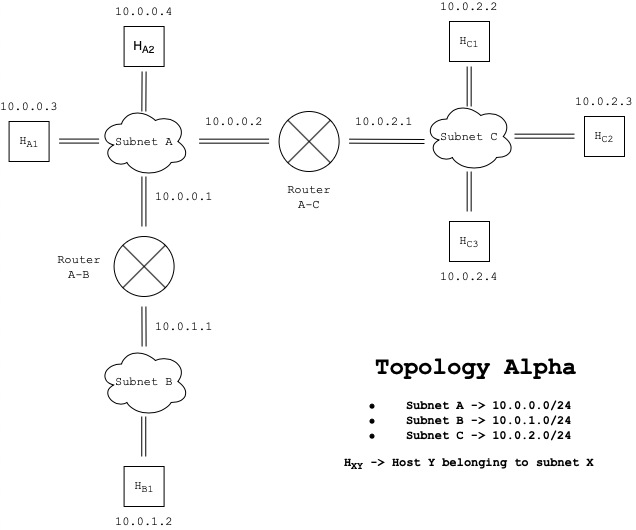
\includegraphics[width=0.75\linewidth]{topology_alpha.png}
                \caption{The \textit{Alpha Topology}.}
                \label{fig:top-alpha}
            \end{figure}

        \subsection{Topology Beta}
            This second topology added another subnet to the previous to push our routing procedures a little further. It is shown on figure \ref{fig:top-beta}.\\

            \begin{figure}
                \centering
                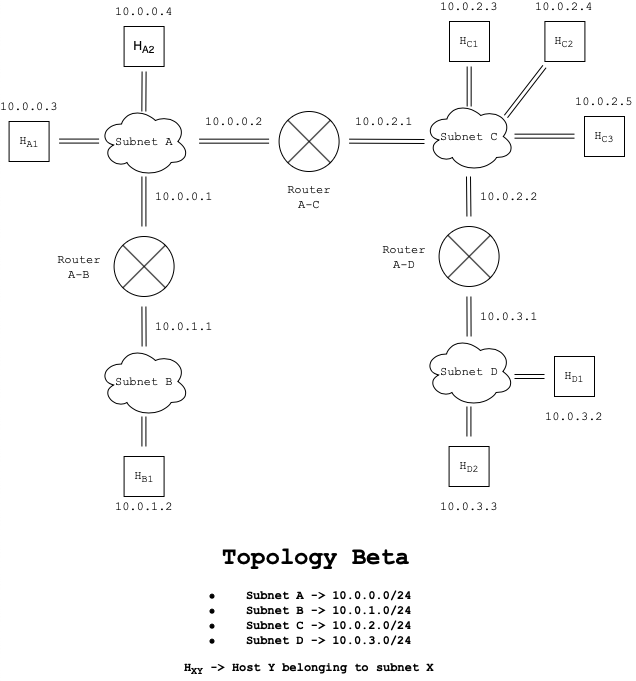
\includegraphics[width=0.75\linewidth]{topology_beta.png}
                \caption{The \textit{Beta Topology}.}
                \label{fig:top-beta}
            \end{figure}

        \subsection{Topology Gamma}
            This third topology, shown on figure \ref{fig:top-gamma}, added yet another subnet to the previous one. After successfully instantiating this topology we felt confident our design was capable of handling significantly more complex topologies.\\

            \begin{figure}
                \centering
                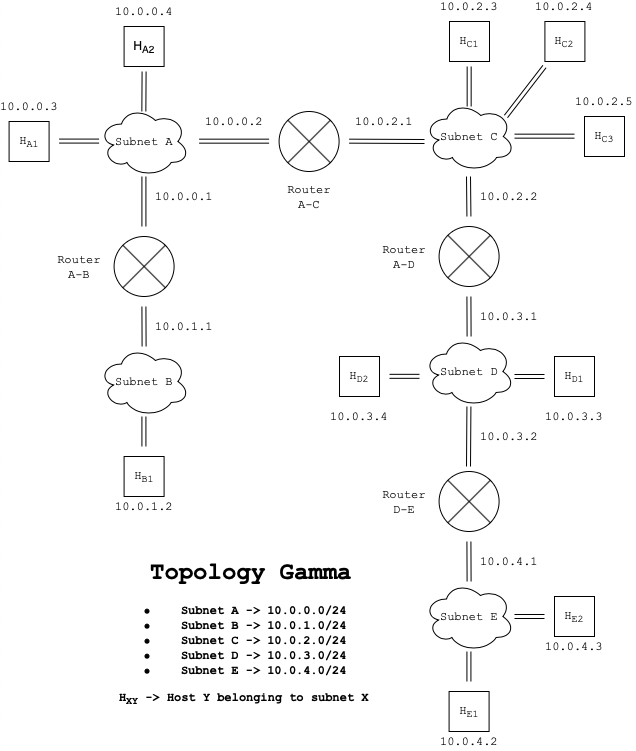
\includegraphics[width=0.75\linewidth]{topology_gamma.png}
                \caption{The \textit{Gamma Topology}.}
                \label{fig:top-gamma}
            \end{figure}

        \subsection{Topology ICS}
            This fourth topology, portrayed on figure \ref{fig:top-ics}, is modeled after \textit{figure 4} of \cite{bib:ics-article}. It is the most complex one we have worked with and the chosen scenario for the proof of concept. We would like to note how, unless otherwise specified \textbf{all the firewalls drop packets} (i.e. only hosts listed on the \textit{FW Conf} sections on figure \ref{fig:top-ics} can communicate).\\

            \begin{figure}
                \centering
                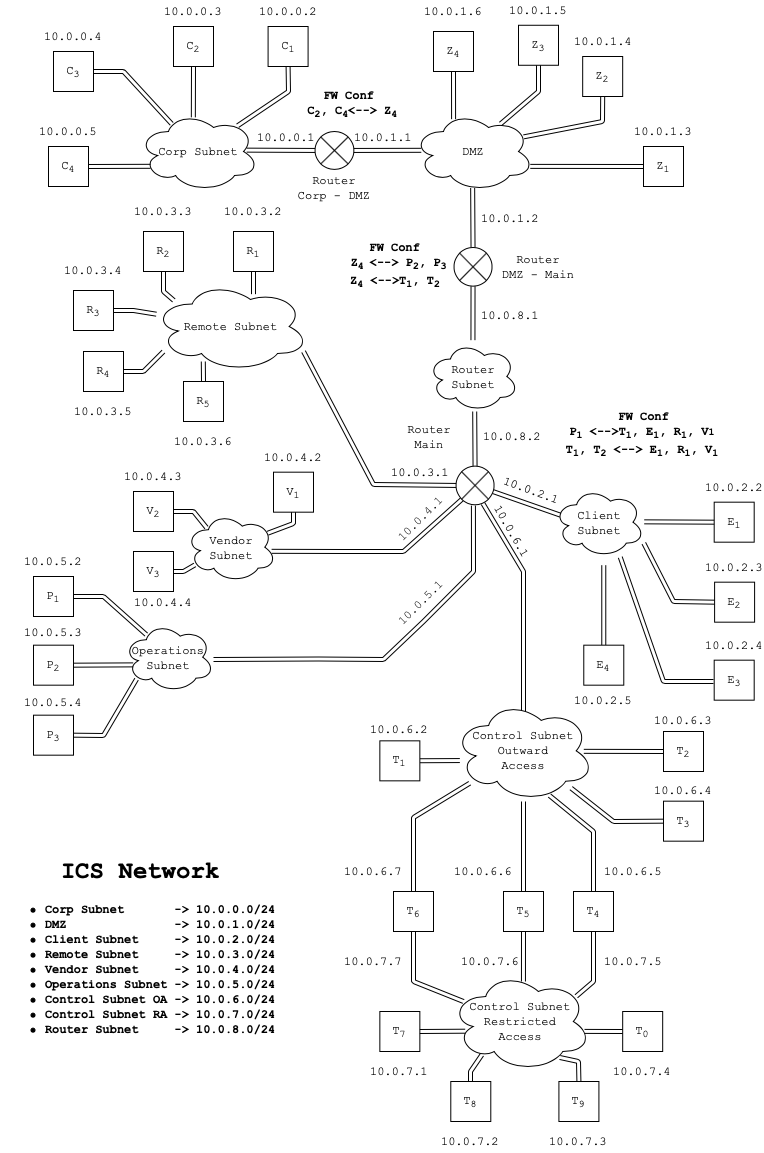
\includegraphics[width=0.75\linewidth]{topology_ics.png}
                \caption{The \textit{ICS (Industrial Control System) Topology}.}
                \label{fig:top-ics}
            \end{figure}
